\documentclass[twoside]{book}

% Packages required by doxygen
\usepackage{fixltx2e}
\usepackage{calc}
\usepackage{doxygen}
\usepackage[export]{adjustbox} % also loads graphicx
\usepackage{graphicx}
\usepackage[utf8]{inputenc}
\usepackage{makeidx}
\usepackage{multicol}
\usepackage{multirow}
\PassOptionsToPackage{warn}{textcomp}
\usepackage{textcomp}
\usepackage[nointegrals]{wasysym}
\usepackage[table]{xcolor}

% Font selection
\usepackage[T1]{fontenc}
\usepackage[scaled=.90]{helvet}
\usepackage{courier}
\usepackage{amssymb}
\usepackage{sectsty}
\renewcommand{\familydefault}{\sfdefault}
\allsectionsfont{%
  \fontseries{bc}\selectfont%
  \color{darkgray}%
}
\renewcommand{\DoxyLabelFont}{%
  \fontseries{bc}\selectfont%
  \color{darkgray}%
}
\newcommand{\+}{\discretionary{\mbox{\scriptsize$\hookleftarrow$}}{}{}}

% Page & text layout
\usepackage{geometry}
\geometry{%
  a4paper,%
  top=2.5cm,%
  bottom=2.5cm,%
  left=2.5cm,%
  right=2.5cm%
}
\tolerance=750
\hfuzz=15pt
\hbadness=750
\setlength{\emergencystretch}{15pt}
\setlength{\parindent}{0cm}
\setlength{\parskip}{3ex plus 2ex minus 2ex}
\makeatletter
\renewcommand{\paragraph}{%
  \@startsection{paragraph}{4}{0ex}{-1.0ex}{1.0ex}{%
    \normalfont\normalsize\bfseries\SS@parafont%
  }%
}
\renewcommand{\subparagraph}{%
  \@startsection{subparagraph}{5}{0ex}{-1.0ex}{1.0ex}{%
    \normalfont\normalsize\bfseries\SS@subparafont%
  }%
}
\makeatother

% Headers & footers
\usepackage{fancyhdr}
\pagestyle{fancyplain}
\fancyhead[LE]{\fancyplain{}{\bfseries\thepage}}
\fancyhead[CE]{\fancyplain{}{}}
\fancyhead[RE]{\fancyplain{}{\bfseries\leftmark}}
\fancyhead[LO]{\fancyplain{}{\bfseries\rightmark}}
\fancyhead[CO]{\fancyplain{}{}}
\fancyhead[RO]{\fancyplain{}{\bfseries\thepage}}
\fancyfoot[LE]{\fancyplain{}{}}
\fancyfoot[CE]{\fancyplain{}{}}
\fancyfoot[RE]{\fancyplain{}{\bfseries\scriptsize Generated by Doxygen }}
\fancyfoot[LO]{\fancyplain{}{\bfseries\scriptsize Generated by Doxygen }}
\fancyfoot[CO]{\fancyplain{}{}}
\fancyfoot[RO]{\fancyplain{}{}}
\renewcommand{\footrulewidth}{0.4pt}
\renewcommand{\chaptermark}[1]{%
  \markboth{#1}{}%
}
\renewcommand{\sectionmark}[1]{%
  \markright{\thesection\ #1}%
}

% Indices & bibliography
\usepackage{natbib}
\usepackage[titles]{tocloft}
\setcounter{tocdepth}{3}
\setcounter{secnumdepth}{5}
\makeindex

% Hyperlinks (required, but should be loaded last)
\usepackage{ifpdf}
\ifpdf
  \usepackage[pdftex,pagebackref=true]{hyperref}
\else
  \usepackage[ps2pdf,pagebackref=true]{hyperref}
\fi
\hypersetup{%
  colorlinks=true,%
  linkcolor=blue,%
  citecolor=blue,%
  unicode%
}

% Custom commands
\newcommand{\clearemptydoublepage}{%
  \newpage{\pagestyle{empty}\cleardoublepage}%
}

\usepackage{caption}
\captionsetup{labelsep=space,justification=centering,font={bf},singlelinecheck=off,skip=4pt,position=top}

%===== C O N T E N T S =====

\begin{document}

% Titlepage & ToC
\hypersetup{pageanchor=false,
             bookmarksnumbered=true,
             pdfencoding=unicode
            }
\pagenumbering{alph}
\begin{titlepage}
\vspace*{7cm}
\begin{center}%
{\Large C\+S\+CE 315\+: People Counter \\[1ex]\large 1.\+0 }\\
\vspace*{1cm}
{\large Generated by Doxygen 1.8.14}\\
\end{center}
\end{titlepage}
\clearemptydoublepage
\pagenumbering{roman}
\tableofcontents
\clearemptydoublepage
\pagenumbering{arabic}
\hypersetup{pageanchor=true}

%--- Begin generated contents ---
\chapter{Hierarchical Index}
\section{Class Hierarchy}
This inheritance list is sorted roughly, but not completely, alphabetically\+:\begin{DoxyCompactList}
\item \contentsline{section}{Data\+Filter.\+Data\+Filter}{\pageref{class_data_filter_1_1_data_filter}}{}
\item object\begin{DoxyCompactList}
\item \contentsline{section}{Sensor\+App.\+Sensor\+App}{\pageref{class_sensor_app_1_1_sensor_app}}{}
\item \contentsline{section}{Server\+App.\+Server\+App}{\pageref{class_server_app_1_1_server_app}}{}
\end{DoxyCompactList}
\end{DoxyCompactList}

\chapter{Class Index}
\section{Class List}
Here are the classes, structs, unions and interfaces with brief descriptions\+:\begin{DoxyCompactList}
\item\contentsline{section}{\mbox{\hyperlink{class_data_filter_1_1_data_filter}{Data\+Filter.\+Data\+Filter}} }{\pageref{class_data_filter_1_1_data_filter}}{}
\item\contentsline{section}{\mbox{\hyperlink{class_sensor_app_1_1_sensor_app}{Sensor\+App.\+Sensor\+App}} \\*Implementation talking to the ranging sensor }{\pageref{class_sensor_app_1_1_sensor_app}}{}
\item\contentsline{section}{\mbox{\hyperlink{class_server_app_1_1_server_app}{Server\+App.\+Server\+App}} }{\pageref{class_server_app_1_1_server_app}}{}
\end{DoxyCompactList}

\chapter{Class Documentation}
\hypertarget{class_data_filter_1_1_data_filter}{}\section{Data\+Filter.\+Data\+Filter Class Reference}
\label{class_data_filter_1_1_data_filter}\index{Data\+Filter.\+Data\+Filter@{Data\+Filter.\+Data\+Filter}}
\subsection*{Public Member Functions}
\begin{DoxyCompactItemize}
\item 
def \mbox{\hyperlink{class_data_filter_1_1_data_filter_ac410f2a7e9574299ee6aff0aff11d3a9}{\+\_\+\+\_\+init\+\_\+\+\_\+}} (self)
\begin{DoxyCompactList}\small\item\em Instantiates Sensor\+App object and sets constants as specified. \end{DoxyCompactList}\item 
\mbox{\Hypertarget{class_data_filter_1_1_data_filter_a57a96ca7f581852e2922be99f48578e5}\label{class_data_filter_1_1_data_filter_a57a96ca7f581852e2922be99f48578e5}} 
def \mbox{\hyperlink{class_data_filter_1_1_data_filter_a57a96ca7f581852e2922be99f48578e5}{read\+Data}} (self)
\begin{DoxyCompactList}\small\item\em Reads latest distance values from Sensor\+App object and updates existing structures within \mbox{\hyperlink{class_data_filter_1_1_data_filter}{Data\+Filter}} class with the new values. \end{DoxyCompactList}\item 
def \mbox{\hyperlink{class_data_filter_1_1_data_filter_a8ce1d7743127e462a018d678d5e44927}{send\+Data}} (self)
\begin{DoxyCompactList}\small\item\em To be called by Server\+App. \end{DoxyCompactList}\item 
def \mbox{\hyperlink{class_data_filter_1_1_data_filter_ae58c36c4343d52baf699c2ce68fbb784}{get\+Data}} (self)
\begin{DoxyCompactList}\small\item\em To be called by Server\+App. \end{DoxyCompactList}\item 
def \mbox{\hyperlink{class_data_filter_1_1_data_filter_a2b121b53a52353af961ce977449e4bfa}{clear\+Data}} (self)
\begin{DoxyCompactList}\small\item\em To be called by Server\+App. \end{DoxyCompactList}\item 
def \mbox{\hyperlink{class_data_filter_1_1_data_filter_a3e2775cb10b099daeb8a7bcf9aa5fe9f}{calibrate}} (self)
\begin{DoxyCompactList}\small\item\em Called by constructor and used to calibrate environment noise to improve the filter\textquotesingle{}s ability to discern legitimate distance values read by the Sensor\+App object. \end{DoxyCompactList}\item 
def \mbox{\hyperlink{class_data_filter_1_1_data_filter_a494edf5de2ab50286063711a120d05ef}{update\+Data}} (self, response)
\begin{DoxyCompactList}\small\item\em Work horse of the \mbox{\hyperlink{class_data_filter_1_1_data_filter}{Data\+Filter}} class. \end{DoxyCompactList}\item 
def \mbox{\hyperlink{class_data_filter_1_1_data_filter_afed5beb108e5fc193a7d8de6b183c047}{make\+Judgement\+Call}} (self, item, \mbox{\hyperlink{class_data_filter_1_1_data_filter_a2f9315bfe6ab0a7b74bcb98310b2f8d2}{sensor}})
\begin{DoxyCompactList}\small\item\em Ultimately determines whether a distance value expired in either expectation buffer should be counted as a person walking in a particular direction. \end{DoxyCompactList}\end{DoxyCompactItemize}
\subsection*{Static Public Attributes}
\begin{DoxyCompactItemize}
\item 
\mbox{\Hypertarget{class_data_filter_1_1_data_filter_a60f284188457f923012772e742b80fea}\label{class_data_filter_1_1_data_filter_a60f284188457f923012772e742b80fea}} 
\mbox{\hyperlink{class_data_filter_1_1_data_filter_a60f284188457f923012772e742b80fea}{people\+Counted}}
\begin{DoxyCompactList}\small\item\em Object\textquotesingle{}s local count for number of pedestrians. \end{DoxyCompactList}\item 
\mbox{\Hypertarget{class_data_filter_1_1_data_filter_acf552ffa41362c83cb122789fe773329}\label{class_data_filter_1_1_data_filter_acf552ffa41362c83cb122789fe773329}} 
\mbox{\hyperlink{class_data_filter_1_1_data_filter_acf552ffa41362c83cb122789fe773329}{num\+Readings}}
\begin{DoxyCompactList}\small\item\em The number of readings we want from the sensor each cycle. \end{DoxyCompactList}\item 
\mbox{\Hypertarget{class_data_filter_1_1_data_filter_a2f9315bfe6ab0a7b74bcb98310b2f8d2}\label{class_data_filter_1_1_data_filter_a2f9315bfe6ab0a7b74bcb98310b2f8d2}} 
\mbox{\hyperlink{class_data_filter_1_1_data_filter_a2f9315bfe6ab0a7b74bcb98310b2f8d2}{sensor}}
\begin{DoxyCompactList}\small\item\em Initializing Sensor\+App object. \end{DoxyCompactList}\item 
\mbox{\Hypertarget{class_data_filter_1_1_data_filter_a2d139273025a1cb06007c3a5b43f084e}\label{class_data_filter_1_1_data_filter_a2d139273025a1cb06007c3a5b43f084e}} 
\mbox{\hyperlink{class_data_filter_1_1_data_filter_a2d139273025a1cb06007c3a5b43f084e}{s1\+Data}}
\begin{DoxyCompactList}\small\item\em Structure to store latest distance values read by sensor 1. \end{DoxyCompactList}\item 
\mbox{\Hypertarget{class_data_filter_1_1_data_filter_a8c4508633e4146d7552e7cc7a8329717}\label{class_data_filter_1_1_data_filter_a8c4508633e4146d7552e7cc7a8329717}} 
\mbox{\hyperlink{class_data_filter_1_1_data_filter_a8c4508633e4146d7552e7cc7a8329717}{s2\+Data}}
\begin{DoxyCompactList}\small\item\em Structure to store latest distance values read by sensor 2. \end{DoxyCompactList}\item 
\mbox{\Hypertarget{class_data_filter_1_1_data_filter_a366cd6f9f50cb14b36c4db06520acd1b}\label{class_data_filter_1_1_data_filter_a366cd6f9f50cb14b36c4db06520acd1b}} 
\mbox{\hyperlink{class_data_filter_1_1_data_filter_a366cd6f9f50cb14b36c4db06520acd1b}{E\+B\+S1}}
\begin{DoxyCompactList}\small\item\em Expectation buffer for sensor 1; stores distance values, timestamps, and other relevant info. \end{DoxyCompactList}\item 
\mbox{\Hypertarget{class_data_filter_1_1_data_filter_ae4f6d96d9cf2726c077d31a0457009c5}\label{class_data_filter_1_1_data_filter_ae4f6d96d9cf2726c077d31a0457009c5}} 
\mbox{\hyperlink{class_data_filter_1_1_data_filter_ae4f6d96d9cf2726c077d31a0457009c5}{E\+B\+S2}}
\begin{DoxyCompactList}\small\item\em Expectation buffer for sensor 2. \end{DoxyCompactList}\item 
\mbox{\Hypertarget{class_data_filter_1_1_data_filter_a995c23055bc575f0fa3cf25584ca2f97}\label{class_data_filter_1_1_data_filter_a995c23055bc575f0fa3cf25584ca2f97}} 
\mbox{\hyperlink{class_data_filter_1_1_data_filter_a995c23055bc575f0fa3cf25584ca2f97}{noise}}
\begin{DoxyCompactList}\small\item\em Depth of environment to determine upper bound on legitimate distance readings. \end{DoxyCompactList}\item 
\mbox{\Hypertarget{class_data_filter_1_1_data_filter_aed08d319cdf84ec98cc220bb866695da}\label{class_data_filter_1_1_data_filter_aed08d319cdf84ec98cc220bb866695da}} 
\mbox{\hyperlink{class_data_filter_1_1_data_filter_aed08d319cdf84ec98cc220bb866695da}{time\+Buffer}}
\begin{DoxyCompactList}\small\item\em Range of time beyond which we conclude separate people triggered sensor. \end{DoxyCompactList}\item 
\mbox{\Hypertarget{class_data_filter_1_1_data_filter_a54efa3bad5ef62cbd98b4a54303f70a6}\label{class_data_filter_1_1_data_filter_a54efa3bad5ef62cbd98b4a54303f70a6}} 
\mbox{\hyperlink{class_data_filter_1_1_data_filter_a54efa3bad5ef62cbd98b4a54303f70a6}{distance\+Buffer}}
\begin{DoxyCompactList}\small\item\em Range of distance beyond which we conclude separate people triggered sensor. \end{DoxyCompactList}\end{DoxyCompactItemize}


\subsection{Constructor \& Destructor Documentation}
\mbox{\Hypertarget{class_data_filter_1_1_data_filter_ac410f2a7e9574299ee6aff0aff11d3a9}\label{class_data_filter_1_1_data_filter_ac410f2a7e9574299ee6aff0aff11d3a9}} 
\index{Data\+Filter\+::\+Data\+Filter@{Data\+Filter\+::\+Data\+Filter}!\+\_\+\+\_\+init\+\_\+\+\_\+@{\+\_\+\+\_\+init\+\_\+\+\_\+}}
\index{\+\_\+\+\_\+init\+\_\+\+\_\+@{\+\_\+\+\_\+init\+\_\+\+\_\+}!Data\+Filter\+::\+Data\+Filter@{Data\+Filter\+::\+Data\+Filter}}
\subsubsection{\texorpdfstring{\+\_\+\+\_\+init\+\_\+\+\_\+()}{\_\_init\_\_()}}
{\footnotesize\ttfamily def Data\+Filter.\+Data\+Filter.\+\_\+\+\_\+init\+\_\+\+\_\+ (\begin{DoxyParamCaption}\item[{}]{self }\end{DoxyParamCaption})}



Instantiates Sensor\+App object and sets constants as specified. 

Calibrates environment noise. 

\subsection{Member Function Documentation}
\mbox{\Hypertarget{class_data_filter_1_1_data_filter_a3e2775cb10b099daeb8a7bcf9aa5fe9f}\label{class_data_filter_1_1_data_filter_a3e2775cb10b099daeb8a7bcf9aa5fe9f}} 
\index{Data\+Filter\+::\+Data\+Filter@{Data\+Filter\+::\+Data\+Filter}!calibrate@{calibrate}}
\index{calibrate@{calibrate}!Data\+Filter\+::\+Data\+Filter@{Data\+Filter\+::\+Data\+Filter}}
\subsubsection{\texorpdfstring{calibrate()}{calibrate()}}
{\footnotesize\ttfamily def Data\+Filter.\+Data\+Filter.\+calibrate (\begin{DoxyParamCaption}\item[{}]{self }\end{DoxyParamCaption})}



Called by constructor and used to calibrate environment noise to improve the filter\textquotesingle{}s ability to discern legitimate distance values read by the Sensor\+App object. 

\begin{DoxyReturn}{Returns}
Calibrated background noise with which distance readings from both sensors are compared 
\end{DoxyReturn}
\mbox{\Hypertarget{class_data_filter_1_1_data_filter_a2b121b53a52353af961ce977449e4bfa}\label{class_data_filter_1_1_data_filter_a2b121b53a52353af961ce977449e4bfa}} 
\index{Data\+Filter\+::\+Data\+Filter@{Data\+Filter\+::\+Data\+Filter}!clear\+Data@{clear\+Data}}
\index{clear\+Data@{clear\+Data}!Data\+Filter\+::\+Data\+Filter@{Data\+Filter\+::\+Data\+Filter}}
\subsubsection{\texorpdfstring{clear\+Data()}{clearData()}}
{\footnotesize\ttfamily def Data\+Filter.\+Data\+Filter.\+clear\+Data (\begin{DoxyParamCaption}\item[{}]{self }\end{DoxyParamCaption})}



To be called by Server\+App. 

Resets existing number of people counted to 0. \mbox{\Hypertarget{class_data_filter_1_1_data_filter_ae58c36c4343d52baf699c2ce68fbb784}\label{class_data_filter_1_1_data_filter_ae58c36c4343d52baf699c2ce68fbb784}} 
\index{Data\+Filter\+::\+Data\+Filter@{Data\+Filter\+::\+Data\+Filter}!get\+Data@{get\+Data}}
\index{get\+Data@{get\+Data}!Data\+Filter\+::\+Data\+Filter@{Data\+Filter\+::\+Data\+Filter}}
\subsubsection{\texorpdfstring{get\+Data()}{getData()}}
{\footnotesize\ttfamily def Data\+Filter.\+Data\+Filter.\+get\+Data (\begin{DoxyParamCaption}\item[{}]{self }\end{DoxyParamCaption})}



To be called by Server\+App. 

Returns existing number of people counted.

\begin{DoxyReturn}{Returns}
Existing local count of \mbox{\hyperlink{class_data_filter_1_1_data_filter}{Data\+Filter}} object 
\end{DoxyReturn}
\mbox{\Hypertarget{class_data_filter_1_1_data_filter_afed5beb108e5fc193a7d8de6b183c047}\label{class_data_filter_1_1_data_filter_afed5beb108e5fc193a7d8de6b183c047}} 
\index{Data\+Filter\+::\+Data\+Filter@{Data\+Filter\+::\+Data\+Filter}!make\+Judgement\+Call@{make\+Judgement\+Call}}
\index{make\+Judgement\+Call@{make\+Judgement\+Call}!Data\+Filter\+::\+Data\+Filter@{Data\+Filter\+::\+Data\+Filter}}
\subsubsection{\texorpdfstring{make\+Judgement\+Call()}{makeJudgementCall()}}
{\footnotesize\ttfamily def Data\+Filter.\+Data\+Filter.\+make\+Judgement\+Call (\begin{DoxyParamCaption}\item[{}]{self,  }\item[{}]{item,  }\item[{}]{sensor }\end{DoxyParamCaption})}



Ultimately determines whether a distance value expired in either expectation buffer should be counted as a person walking in a particular direction. 


\begin{DoxyParams}{Parameters}
{\em item} & an element of the expectation buffer \\
\hline
{\em sensor} & is the number of the sensor (in this case we only support 2 sensors) \\
\hline
\end{DoxyParams}
\mbox{\Hypertarget{class_data_filter_1_1_data_filter_a8ce1d7743127e462a018d678d5e44927}\label{class_data_filter_1_1_data_filter_a8ce1d7743127e462a018d678d5e44927}} 
\index{Data\+Filter\+::\+Data\+Filter@{Data\+Filter\+::\+Data\+Filter}!send\+Data@{send\+Data}}
\index{send\+Data@{send\+Data}!Data\+Filter\+::\+Data\+Filter@{Data\+Filter\+::\+Data\+Filter}}
\subsubsection{\texorpdfstring{send\+Data()}{sendData()}}
{\footnotesize\ttfamily def Data\+Filter.\+Data\+Filter.\+send\+Data (\begin{DoxyParamCaption}\item[{}]{self }\end{DoxyParamCaption})}



To be called by Server\+App. 

Returns existing number of people counted and resets value to 0. \begin{DoxyReturn}{Returns}
Number of peoplecounted 
\end{DoxyReturn}
\mbox{\Hypertarget{class_data_filter_1_1_data_filter_a494edf5de2ab50286063711a120d05ef}\label{class_data_filter_1_1_data_filter_a494edf5de2ab50286063711a120d05ef}} 
\index{Data\+Filter\+::\+Data\+Filter@{Data\+Filter\+::\+Data\+Filter}!update\+Data@{update\+Data}}
\index{update\+Data@{update\+Data}!Data\+Filter\+::\+Data\+Filter@{Data\+Filter\+::\+Data\+Filter}}
\subsubsection{\texorpdfstring{update\+Data()}{updateData()}}
{\footnotesize\ttfamily def Data\+Filter.\+Data\+Filter.\+update\+Data (\begin{DoxyParamCaption}\item[{}]{self,  }\item[{}]{response }\end{DoxyParamCaption})}



Work horse of the \mbox{\hyperlink{class_data_filter_1_1_data_filter}{Data\+Filter}} class. 

Updates existing class structures with new distance values, discerns whether legitimate data has been measured, and makes judgement calls on expired distance values in either expectation buffer.

\begin{DoxyVerb}        A multidimensional array of tuples [ [ (timestamp, distance), ... , (timestamp, distance) ],[ (timestamp, distance), ... , (timestamp, distance) ] ], where each internal array corresponds to a sensor\end{DoxyVerb}
 

The documentation for this class was generated from the following file\+:\begin{DoxyCompactItemize}
\item 
C\+:/\+Users/\+Nicholas/git-\/wkspace/\+C\+S\+C\+E\+\_\+315\+\_\+\+Project\+\_\+\+One/python\+\_\+src/Data\+Filter.\+py\end{DoxyCompactItemize}

\hypertarget{class_sensor_app_1_1_sensor_app}{}\section{Sensor\+App.\+Sensor\+App Class Reference}
\label{class_sensor_app_1_1_sensor_app}\index{Sensor\+App.\+Sensor\+App@{Sensor\+App.\+Sensor\+App}}


Implementation talking to the ranging sensor.  




Inheritance diagram for Sensor\+App.\+Sensor\+App\+:
\nopagebreak
\begin{figure}[H]
\begin{center}
\leavevmode
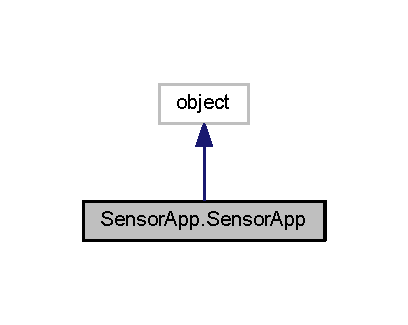
\includegraphics[width=196pt]{class_sensor_app_1_1_sensor_app__inherit__graph}
\end{center}
\end{figure}
\subsection*{Public Member Functions}
\begin{DoxyCompactItemize}
\item 
def \mbox{\hyperlink{class_sensor_app_1_1_sensor_app_ad925f61b0da07144eda6b3d313087d2e}{\+\_\+\+\_\+init\+\_\+\+\_\+}} (self, \mbox{\hyperlink{class_sensor_app_1_1_sensor_app_a888dda7b7c27cafa37ed670114bf1c9b}{arduino\+\_\+port}}, \mbox{\hyperlink{class_sensor_app_1_1_sensor_app_a63cf06625f46bb3ac62bead94d06f2b4}{baudrate}}, \mbox{\hyperlink{class_sensor_app_1_1_sensor_app_ad6dfe39d8eb808d881f5a4f76f1b38ac}{update\+\_\+rate}}, \mbox{\hyperlink{class_sensor_app_1_1_sensor_app_a657c2112bb07280d3249eb1f1899affd}{trigger\+\_\+pins}}, \mbox{\hyperlink{class_sensor_app_1_1_sensor_app_a1e393f1f58d859a71a34c53849929e7c}{echo\+\_\+pins}})
\begin{DoxyCompactList}\small\item\em Initializes the \mbox{\hyperlink{class_sensor_app_1_1_sensor_app}{Sensor\+App}} with the given arduino\+\_\+port and the baudrate on that port. \end{DoxyCompactList}\item 
def \mbox{\hyperlink{class_sensor_app_1_1_sensor_app_a59839f70657056c516b4740b610755fa}{configure\+\_\+ard}} (self)
\begin{DoxyCompactList}\small\item\em Configures the arduino with the number of trigger and echo pins as well as the update rate specified in the initialization of the sensor\+App class. \end{DoxyCompactList}\item 
def \mbox{\hyperlink{class_sensor_app_1_1_sensor_app_a6558c7ef5bd20ba3d71bb84b24431853}{read\+From\+Serial}} (self, msg\+\_\+length)
\begin{DoxyCompactList}\small\item\em Encapsulates the reading from the serial socket and conversion to A\+S\+C\+II to make this more digestable. \end{DoxyCompactList}\item 
def \mbox{\hyperlink{class_sensor_app_1_1_sensor_app_a77bcd8b2f4f3bf1c55e8c7fa105edf46}{send\+To\+Serial}} (self, msg)
\begin{DoxyCompactList}\small\item\em Helper function to convert the characters to ascii encoding so that the Arduino can understand them. \end{DoxyCompactList}\item 
def \mbox{\hyperlink{class_sensor_app_1_1_sensor_app_aae2bb034ebfed964fa17fef43dddc8da}{read\+From\+Sensor}} (self, nbr\+Readings=5)
\begin{DoxyCompactList}\small\item\em Reads the number of readings specified by nbr\+Readings from the sensor. \end{DoxyCompactList}\item 
def \mbox{\hyperlink{class_sensor_app_1_1_sensor_app_a71471ab0e8fd7c112008232d21282df5}{print\+Pretty\+Response}} (self, resp)
\begin{DoxyCompactList}\small\item\em Helper function for debugging. \end{DoxyCompactList}\end{DoxyCompactItemize}
\subsection*{Public Attributes}
\begin{DoxyCompactItemize}
\item 
\mbox{\Hypertarget{class_sensor_app_1_1_sensor_app_a888dda7b7c27cafa37ed670114bf1c9b}\label{class_sensor_app_1_1_sensor_app_a888dda7b7c27cafa37ed670114bf1c9b}} 
\mbox{\hyperlink{class_sensor_app_1_1_sensor_app_a888dda7b7c27cafa37ed670114bf1c9b}{arduino\+\_\+port}}
\begin{DoxyCompactList}\small\item\em Port for the Arduino to connect to. \end{DoxyCompactList}\item 
\mbox{\Hypertarget{class_sensor_app_1_1_sensor_app_a63cf06625f46bb3ac62bead94d06f2b4}\label{class_sensor_app_1_1_sensor_app_a63cf06625f46bb3ac62bead94d06f2b4}} 
\mbox{\hyperlink{class_sensor_app_1_1_sensor_app_a63cf06625f46bb3ac62bead94d06f2b4}{baudrate}}
\begin{DoxyCompactList}\small\item\em Baudrate of the arduino\+\_\+port, should be 250000. \end{DoxyCompactList}\item 
\mbox{\Hypertarget{class_sensor_app_1_1_sensor_app_aef6da161ddb54a90905a9cb8d793d9de}\label{class_sensor_app_1_1_sensor_app_aef6da161ddb54a90905a9cb8d793d9de}} 
\mbox{\hyperlink{class_sensor_app_1_1_sensor_app_aef6da161ddb54a90905a9cb8d793d9de}{sock}}
\begin{DoxyCompactList}\small\item\em Serial Socket created to communicate with the arduino over the arduino\+\_\+port. \end{DoxyCompactList}\item 
\mbox{\Hypertarget{class_sensor_app_1_1_sensor_app_ad6dfe39d8eb808d881f5a4f76f1b38ac}\label{class_sensor_app_1_1_sensor_app_ad6dfe39d8eb808d881f5a4f76f1b38ac}} 
\mbox{\hyperlink{class_sensor_app_1_1_sensor_app_ad6dfe39d8eb808d881f5a4f76f1b38ac}{update\+\_\+rate}}
\begin{DoxyCompactList}\small\item\em Specified update\+\_\+rate for the arduino. \end{DoxyCompactList}\item 
\mbox{\Hypertarget{class_sensor_app_1_1_sensor_app_a657c2112bb07280d3249eb1f1899affd}\label{class_sensor_app_1_1_sensor_app_a657c2112bb07280d3249eb1f1899affd}} 
\mbox{\hyperlink{class_sensor_app_1_1_sensor_app_a657c2112bb07280d3249eb1f1899affd}{trigger\+\_\+pins}}
\begin{DoxyCompactList}\small\item\em Pins for triggering the ultrasonic sensor. \end{DoxyCompactList}\item 
\mbox{\Hypertarget{class_sensor_app_1_1_sensor_app_a1e393f1f58d859a71a34c53849929e7c}\label{class_sensor_app_1_1_sensor_app_a1e393f1f58d859a71a34c53849929e7c}} 
\mbox{\hyperlink{class_sensor_app_1_1_sensor_app_a1e393f1f58d859a71a34c53849929e7c}{echo\+\_\+pins}}
\begin{DoxyCompactList}\small\item\em Pins for the echo signal on the ultrasonic sensor. \end{DoxyCompactList}\end{DoxyCompactItemize}


\subsection{Detailed Description}
Implementation talking to the ranging sensor. 

Encaspulates the configuration and communication with the sensor using custom configuration protocol. This class needs to be used in conjunction with the firmware held inside of the Arduino directory 

\subsection{Constructor \& Destructor Documentation}
\mbox{\Hypertarget{class_sensor_app_1_1_sensor_app_ad925f61b0da07144eda6b3d313087d2e}\label{class_sensor_app_1_1_sensor_app_ad925f61b0da07144eda6b3d313087d2e}} 
\index{Sensor\+App\+::\+Sensor\+App@{Sensor\+App\+::\+Sensor\+App}!\+\_\+\+\_\+init\+\_\+\+\_\+@{\+\_\+\+\_\+init\+\_\+\+\_\+}}
\index{\+\_\+\+\_\+init\+\_\+\+\_\+@{\+\_\+\+\_\+init\+\_\+\+\_\+}!Sensor\+App\+::\+Sensor\+App@{Sensor\+App\+::\+Sensor\+App}}
\subsubsection{\texorpdfstring{\+\_\+\+\_\+init\+\_\+\+\_\+()}{\_\_init\_\_()}}
{\footnotesize\ttfamily def Sensor\+App.\+Sensor\+App.\+\_\+\+\_\+init\+\_\+\+\_\+ (\begin{DoxyParamCaption}\item[{}]{self,  }\item[{}]{arduino\+\_\+port,  }\item[{}]{baudrate,  }\item[{}]{update\+\_\+rate,  }\item[{}]{trigger\+\_\+pins,  }\item[{}]{echo\+\_\+pins }\end{DoxyParamCaption})}



Initializes the \mbox{\hyperlink{class_sensor_app_1_1_sensor_app}{Sensor\+App}} with the given arduino\+\_\+port and the baudrate on that port. 


\begin{DoxyParams}{Parameters}
{\em arduino\+\_\+port} & port to communicate to the arduino over \\
\hline
{\em baudrate} & baudrate of the arduino\+\_\+port, for our application we set it to 250k\+Hz, but if you change the the baudrate in the firmware you need to change this aswell \\
\hline
{\em update\+\_\+rate} & update rate that the arduino will be set to \\
\hline
{\em trigger\+\_\+pins} & An array of the trigger pins that is the same length as the echo\+\_\+pins \\
\hline
{\em echo\+\_\+pins} & An array of the echo\+\_\+pins that is the same length as the trigger\+\_\+pins \\
\hline
\end{DoxyParams}


\subsection{Member Function Documentation}
\mbox{\Hypertarget{class_sensor_app_1_1_sensor_app_a59839f70657056c516b4740b610755fa}\label{class_sensor_app_1_1_sensor_app_a59839f70657056c516b4740b610755fa}} 
\index{Sensor\+App\+::\+Sensor\+App@{Sensor\+App\+::\+Sensor\+App}!configure\+\_\+ard@{configure\+\_\+ard}}
\index{configure\+\_\+ard@{configure\+\_\+ard}!Sensor\+App\+::\+Sensor\+App@{Sensor\+App\+::\+Sensor\+App}}
\subsubsection{\texorpdfstring{configure\+\_\+ard()}{configure\_ard()}}
{\footnotesize\ttfamily def Sensor\+App.\+Sensor\+App.\+configure\+\_\+ard (\begin{DoxyParamCaption}\item[{}]{self }\end{DoxyParamCaption})}



Configures the arduino with the number of trigger and echo pins as well as the update rate specified in the initialization of the sensor\+App class. 

We create the configuration string, send it, and then wait for the S\+U\+CC key to be returned which indicates that the Arduino has been properly configured. There is no error checking here and it is intentionally made so that the program hangs. If no configuration comes back the sensor should not be run. \mbox{\Hypertarget{class_sensor_app_1_1_sensor_app_a71471ab0e8fd7c112008232d21282df5}\label{class_sensor_app_1_1_sensor_app_a71471ab0e8fd7c112008232d21282df5}} 
\index{Sensor\+App\+::\+Sensor\+App@{Sensor\+App\+::\+Sensor\+App}!print\+Pretty\+Response@{print\+Pretty\+Response}}
\index{print\+Pretty\+Response@{print\+Pretty\+Response}!Sensor\+App\+::\+Sensor\+App@{Sensor\+App\+::\+Sensor\+App}}
\subsubsection{\texorpdfstring{print\+Pretty\+Response()}{printPrettyResponse()}}
{\footnotesize\ttfamily def Sensor\+App.\+Sensor\+App.\+print\+Pretty\+Response (\begin{DoxyParamCaption}\item[{}]{self,  }\item[{}]{resp }\end{DoxyParamCaption})}



Helper function for debugging. 

Prints better looking responses that make it easier to read the data \mbox{\Hypertarget{class_sensor_app_1_1_sensor_app_aae2bb034ebfed964fa17fef43dddc8da}\label{class_sensor_app_1_1_sensor_app_aae2bb034ebfed964fa17fef43dddc8da}} 
\index{Sensor\+App\+::\+Sensor\+App@{Sensor\+App\+::\+Sensor\+App}!read\+From\+Sensor@{read\+From\+Sensor}}
\index{read\+From\+Sensor@{read\+From\+Sensor}!Sensor\+App\+::\+Sensor\+App@{Sensor\+App\+::\+Sensor\+App}}
\subsubsection{\texorpdfstring{read\+From\+Sensor()}{readFromSensor()}}
{\footnotesize\ttfamily def Sensor\+App.\+Sensor\+App.\+read\+From\+Sensor (\begin{DoxyParamCaption}\item[{}]{self,  }\item[{}]{nbr\+Readings = {\ttfamily 5} }\end{DoxyParamCaption})}



Reads the number of readings specified by nbr\+Readings from the sensor. 

Returns an array that is of the following format\+:\+: \mbox{[}\mbox{[}Sensor\mbox{]}\mbox{[}Sensor\mbox{]}\mbox{[}Sensor\mbox{]}\mbox{]} Where Sensor is an array of tuples which contain the timestamps at which they where taken and the readings \mbox{[}(TS,RD),(TS,RD),(TS,RD)\mbox{]}. So an exampe of a returned value would be \mbox{[}\mbox{[}(123,456)\mbox{]},\mbox{[}(456,323)\mbox{]},\mbox{[}(765,345)\mbox{]}\mbox{]} Accessign the readings of Sensor one would then be return\+V\+Alue\mbox{[}0\mbox{]}\mbox{[}0\mbox{]}\mbox{[}1\mbox{]} Where the first 0 is the sensor, the second thr reading and the last index should be 0 or 1 where 0 is the timestamp and 1 is the reading. \begin{DoxyVerb}   If you are interested in the format of the communication protocol you need to look at the top of the page or look inside of the documentation for the firmware where you can find the back and forth protocol laid out for you. If the value returned from the sensor is erroneous or there is a bad sync on the socket we will return a fasle value of:: [[(999999999,40000)],[(999999999,40000)]] whcih will be filtered out by our dataFilter. If you need to double check this value just check if the returned reading is over the max of the sensor which is 800.
\end{DoxyVerb}



\begin{DoxyParams}{Parameters}
{\em nbr\+Readings} & number of readings to be returned by the sensor\\
\hline
\end{DoxyParams}
\begin{DoxyReturn}{Returns}
An array of array of tuples where the tuples are of type (Timestamp, Reading) and the array indexes are Sensor and reading number in that order or in the case of failure \mbox{[}\mbox{[}(999999999,40000)\mbox{]},\mbox{[}(999999999,40000)\mbox{]}\mbox{]} 
\end{DoxyReturn}
\mbox{\Hypertarget{class_sensor_app_1_1_sensor_app_a6558c7ef5bd20ba3d71bb84b24431853}\label{class_sensor_app_1_1_sensor_app_a6558c7ef5bd20ba3d71bb84b24431853}} 
\index{Sensor\+App\+::\+Sensor\+App@{Sensor\+App\+::\+Sensor\+App}!read\+From\+Serial@{read\+From\+Serial}}
\index{read\+From\+Serial@{read\+From\+Serial}!Sensor\+App\+::\+Sensor\+App@{Sensor\+App\+::\+Sensor\+App}}
\subsubsection{\texorpdfstring{read\+From\+Serial()}{readFromSerial()}}
{\footnotesize\ttfamily def Sensor\+App.\+Sensor\+App.\+read\+From\+Serial (\begin{DoxyParamCaption}\item[{}]{self,  }\item[{}]{msg\+\_\+length }\end{DoxyParamCaption})}



Encapsulates the reading from the serial socket and conversion to A\+S\+C\+II to make this more digestable. 


\begin{DoxyParams}{Parameters}
{\em msg\+\_\+length} & length of the message to read from the buffer. If the requested message length is longer than the currently available data then only the currently available data is returns\\
\hline
\end{DoxyParams}
\begin{DoxyReturn}{Returns}
An ascii encoded string of the data on the bus of length msg\+\_\+length or sock.\+in\+\_\+waiting 
\end{DoxyReturn}
\mbox{\Hypertarget{class_sensor_app_1_1_sensor_app_a77bcd8b2f4f3bf1c55e8c7fa105edf46}\label{class_sensor_app_1_1_sensor_app_a77bcd8b2f4f3bf1c55e8c7fa105edf46}} 
\index{Sensor\+App\+::\+Sensor\+App@{Sensor\+App\+::\+Sensor\+App}!send\+To\+Serial@{send\+To\+Serial}}
\index{send\+To\+Serial@{send\+To\+Serial}!Sensor\+App\+::\+Sensor\+App@{Sensor\+App\+::\+Sensor\+App}}
\subsubsection{\texorpdfstring{send\+To\+Serial()}{sendToSerial()}}
{\footnotesize\ttfamily def Sensor\+App.\+Sensor\+App.\+send\+To\+Serial (\begin{DoxyParamCaption}\item[{}]{self,  }\item[{}]{msg }\end{DoxyParamCaption})}



Helper function to convert the characters to ascii encoding so that the Arduino can understand them. 

If the msg is of type string then this function will write it to the serial socket and return the number of bytes written otherwise it will return the None type


\begin{DoxyParams}{Parameters}
{\em msg} & msg to be sent over the serial socket\\
\hline
\end{DoxyParams}
\begin{DoxyReturn}{Returns}
None if the message is not of type string or the amount of characters written to the socket 
\end{DoxyReturn}


The documentation for this class was generated from the following file\+:\begin{DoxyCompactItemize}
\item 
C\+:/\+Users/\+Nicholas/git-\/wkspace/\+C\+S\+C\+E\+\_\+315\+\_\+\+Project\+\_\+\+One/python\+\_\+src/Sensor\+App.\+py\end{DoxyCompactItemize}

\hypertarget{class_server_app_1_1_server_app}{}\section{Server\+App.\+Server\+App Class Reference}
\label{class_server_app_1_1_server_app}\index{Server\+App.\+Server\+App@{Server\+App.\+Server\+App}}


Inheritance diagram for Server\+App.\+Server\+App\+:\nopagebreak
\begin{figure}[H]
\begin{center}
\leavevmode
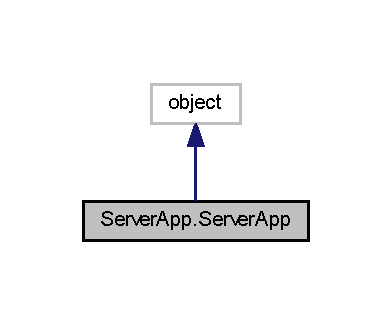
\includegraphics[width=188pt]{class_server_app_1_1_server_app__inherit__graph}
\end{center}
\end{figure}
\subsection*{Public Member Functions}
\begin{DoxyCompactItemize}
\item 
def \mbox{\hyperlink{class_server_app_1_1_server_app_ad21d376322b7fed132f39b87d23ccaea}{\+\_\+\+\_\+init\+\_\+\+\_\+}} (self, \mbox{\hyperlink{class_server_app_1_1_server_app_af133cccb1424b84b45c97e9d03471d17}{db\+\_\+host}}, \mbox{\hyperlink{class_server_app_1_1_server_app_a4fbf66ec391567038cfb6dad6d929708}{db\+\_\+name}}, \mbox{\hyperlink{class_server_app_1_1_server_app_a2991ea2a13aedd112c170df7f5a49265}{db\+\_\+user}}, \mbox{\hyperlink{class_server_app_1_1_server_app_ae409845095d3454690497af61592b3e9}{db\+\_\+pass}}, \mbox{\hyperlink{class_server_app_1_1_server_app_a759e0eaa4be95b98b3c5be7d7fa2eb6e}{db\+\_\+table}}, \mbox{\hyperlink{class_server_app_1_1_server_app_a541e00ca3089461e9ee7f02b3a1fdea9}{db\+Connection}}=True)
\begin{DoxyCompactList}\small\item\em Constructor for the \mbox{\hyperlink{class_server_app_1_1_server_app}{Server\+App}} class. \end{DoxyCompactList}\item 
def \mbox{\hyperlink{class_server_app_1_1_server_app_a4008e39a65dde07e7e69c2eef0b0f578}{connect\+To\+Db}} (self)
\begin{DoxyCompactList}\small\item\em Runs the \+\_\+mysql.\+connect() function to connect to the database. \end{DoxyCompactList}\item 
def \mbox{\hyperlink{class_server_app_1_1_server_app_a665a6527552ef9b8ba12e196b9884655}{set\+Count}} (self, value)
\begin{DoxyCompactList}\small\item\em Set the count amount using the thread safe mutex. \end{DoxyCompactList}\item 
def \mbox{\hyperlink{class_server_app_1_1_server_app_a5b6f47399a9434d1a3b86f89a114a44c}{get\+Count}} (self)
\begin{DoxyCompactList}\small\item\em Get the count suign the thread safe mutex. \end{DoxyCompactList}\item 
def \mbox{\hyperlink{class_server_app_1_1_server_app_acee9930736fb8b9ff4d1229cfede83e4}{kill\+Server\+And\+Nanny}} (self)
\begin{DoxyCompactList}\small\item\em Stops the execution loop of both the database nanny and the main server app function. \end{DoxyCompactList}\item 
def \mbox{\hyperlink{class_server_app_1_1_server_app_a648c098cf7d409cceb017a196b1d0db3}{update\+Database}} (self)
\begin{DoxyCompactList}\small\item\em Pushes the amount of people that have walked by up to the server. \end{DoxyCompactList}\item 
def \mbox{\hyperlink{class_server_app_1_1_server_app_a847d2ab7b7c525f897d710859f363ab5}{start}} (self)
\begin{DoxyCompactList}\small\item\em Start the nanny thread and then begin reading from the sensor via the Data\+Filter. \end{DoxyCompactList}\end{DoxyCompactItemize}
\subsection*{Public Attributes}
\begin{DoxyCompactItemize}
\item 
\mbox{\Hypertarget{class_server_app_1_1_server_app_af133cccb1424b84b45c97e9d03471d17}\label{class_server_app_1_1_server_app_af133cccb1424b84b45c97e9d03471d17}} 
\mbox{\hyperlink{class_server_app_1_1_server_app_af133cccb1424b84b45c97e9d03471d17}{db\+\_\+host}}
\begin{DoxyCompactList}\small\item\em host for the database \end{DoxyCompactList}\item 
\mbox{\Hypertarget{class_server_app_1_1_server_app_a2991ea2a13aedd112c170df7f5a49265}\label{class_server_app_1_1_server_app_a2991ea2a13aedd112c170df7f5a49265}} 
\mbox{\hyperlink{class_server_app_1_1_server_app_a2991ea2a13aedd112c170df7f5a49265}{db\+\_\+user}}
\begin{DoxyCompactList}\small\item\em username for the database \end{DoxyCompactList}\item 
\mbox{\Hypertarget{class_server_app_1_1_server_app_a4fbf66ec391567038cfb6dad6d929708}\label{class_server_app_1_1_server_app_a4fbf66ec391567038cfb6dad6d929708}} 
\mbox{\hyperlink{class_server_app_1_1_server_app_a4fbf66ec391567038cfb6dad6d929708}{db\+\_\+name}}
\begin{DoxyCompactList}\small\item\em name of the database \end{DoxyCompactList}\item 
\mbox{\Hypertarget{class_server_app_1_1_server_app_ae409845095d3454690497af61592b3e9}\label{class_server_app_1_1_server_app_ae409845095d3454690497af61592b3e9}} 
\mbox{\hyperlink{class_server_app_1_1_server_app_ae409845095d3454690497af61592b3e9}{db\+\_\+pass}}
\begin{DoxyCompactList}\small\item\em password for the database \end{DoxyCompactList}\item 
\mbox{\hyperlink{class_server_app_1_1_server_app_a759e0eaa4be95b98b3c5be7d7fa2eb6e}{db\+\_\+table}}
\begin{DoxyCompactList}\small\item\em Table to push data to. \end{DoxyCompactList}\item 
\mbox{\Hypertarget{class_server_app_1_1_server_app_ac135cf1405ae7df3699a2131821af81f}\label{class_server_app_1_1_server_app_ac135cf1405ae7df3699a2131821af81f}} 
\mbox{\hyperlink{class_server_app_1_1_server_app_ac135cf1405ae7df3699a2131821af81f}{sched}}
\begin{DoxyCompactList}\small\item\em Schedular for regularly running the update database. \end{DoxyCompactList}\item 
\mbox{\Hypertarget{class_server_app_1_1_server_app_a392a723730fcdbefd0a4b96f820c9fec}\label{class_server_app_1_1_server_app_a392a723730fcdbefd0a4b96f820c9fec}} 
\mbox{\hyperlink{class_server_app_1_1_server_app_a392a723730fcdbefd0a4b96f820c9fec}{failed\+\_\+queries}}
\begin{DoxyCompactList}\small\item\em Member variable to keep track of the failed queries. \end{DoxyCompactList}\item 
\mbox{\hyperlink{class_server_app_1_1_server_app_a541e00ca3089461e9ee7f02b3a1fdea9}{db\+Connection}}
\begin{DoxyCompactList}\small\item\em Local variable indicating whether to connect to and run the database. \end{DoxyCompactList}\item 
\mbox{\Hypertarget{class_server_app_1_1_server_app_a9749427986bfbdb2428bf5861b61f8c2}\label{class_server_app_1_1_server_app_a9749427986bfbdb2428bf5861b61f8c2}} 
\mbox{\hyperlink{class_server_app_1_1_server_app_a9749427986bfbdb2428bf5861b61f8c2}{count\+\_\+lock}}
\begin{DoxyCompactList}\small\item\em Counter Mutex to keep the database\+Nanny and sensor\+Update threads in sync. \end{DoxyCompactList}\item 
\mbox{\Hypertarget{class_server_app_1_1_server_app_a5a9788c6453de0cb4cfc6a1f82cfa4d1}\label{class_server_app_1_1_server_app_a5a9788c6453de0cb4cfc6a1f82cfa4d1}} 
\mbox{\hyperlink{class_server_app_1_1_server_app_a5a9788c6453de0cb4cfc6a1f82cfa4d1}{kill\+\_\+server}}
\begin{DoxyCompactList}\small\item\em Variable used to kill the database\+Nanny daemon. \end{DoxyCompactList}\item 
\mbox{\Hypertarget{class_server_app_1_1_server_app_a108fcfaa44a437b4a2a8fede99da06ea}\label{class_server_app_1_1_server_app_a108fcfaa44a437b4a2a8fede99da06ea}} 
\mbox{\hyperlink{class_server_app_1_1_server_app_a108fcfaa44a437b4a2a8fede99da06ea}{counted\+\_\+people}}
\begin{DoxyCompactList}\small\item\em The count that is kept of the amount of people that have passed. \end{DoxyCompactList}\item 
\mbox{\Hypertarget{class_server_app_1_1_server_app_a91855cac79a63ea9e2f260d9ae2a6179}\label{class_server_app_1_1_server_app_a91855cac79a63ea9e2f260d9ae2a6179}} 
\mbox{\hyperlink{class_server_app_1_1_server_app_a91855cac79a63ea9e2f260d9ae2a6179}{data\+Filter}}
\begin{DoxyCompactList}\small\item\em Datafulter that determines direction and if people are walking side by side. \end{DoxyCompactList}\item 
\mbox{\hyperlink{class_server_app_1_1_server_app_aa3d45986c6c5a318fe81ec68cb794444}{run}}
\begin{DoxyCompactList}\small\item\em Flag to be set to Flase if we want the \mbox{\hyperlink{class_server_app_1_1_server_app}{Server\+App}} to stop running and kill all it\textquotesingle{}s threads. \end{DoxyCompactList}\item 
\mbox{\Hypertarget{class_server_app_1_1_server_app_a873b13faee0ebe503e91daddf42f013b}\label{class_server_app_1_1_server_app_a873b13faee0ebe503e91daddf42f013b}} 
\mbox{\hyperlink{class_server_app_1_1_server_app_a873b13faee0ebe503e91daddf42f013b}{conn}}
\begin{DoxyCompactList}\small\item\em Connection to the My\+S\+QL db specified by the variables in the constructor (see {\bfseries init} for more detail) \end{DoxyCompactList}\end{DoxyCompactItemize}


\subsection{Constructor \& Destructor Documentation}
\mbox{\Hypertarget{class_server_app_1_1_server_app_ad21d376322b7fed132f39b87d23ccaea}\label{class_server_app_1_1_server_app_ad21d376322b7fed132f39b87d23ccaea}} 
\index{Server\+App\+::\+Server\+App@{Server\+App\+::\+Server\+App}!\+\_\+\+\_\+init\+\_\+\+\_\+@{\+\_\+\+\_\+init\+\_\+\+\_\+}}
\index{\+\_\+\+\_\+init\+\_\+\+\_\+@{\+\_\+\+\_\+init\+\_\+\+\_\+}!Server\+App\+::\+Server\+App@{Server\+App\+::\+Server\+App}}
\subsubsection{\texorpdfstring{\+\_\+\+\_\+init\+\_\+\+\_\+()}{\_\_init\_\_()}}
{\footnotesize\ttfamily def Server\+App.\+Server\+App.\+\_\+\+\_\+init\+\_\+\+\_\+ (\begin{DoxyParamCaption}\item[{}]{self,  }\item[{}]{db\+\_\+host,  }\item[{}]{db\+\_\+name,  }\item[{}]{db\+\_\+user,  }\item[{}]{db\+\_\+pass,  }\item[{}]{db\+\_\+table,  }\item[{}]{db\+Connection = {\ttfamily True} }\end{DoxyParamCaption})}



Constructor for the \mbox{\hyperlink{class_server_app_1_1_server_app}{Server\+App}} class. 

Handles all of the communication between the Data\+Filter and the database specified by the memeber variables above.


\begin{DoxyParams}{Parameters}
{\em db\+\_\+host} & host name for the database to be connected to \\
\hline
{\em db\+\_\+name} & name of the database to be connected to \\
\hline
{\em db\+\_\+user} & username for the database to be connected to \\
\hline
{\em db\+\_\+pass} & password of the database to be connected to \\
\hline
{\em db\+\_\+table} & table to push the data to \\
\hline
{\em db\+Connection} & to connect to the database or not to connect to the database that is the use of this variable \\
\hline
\end{DoxyParams}


\subsection{Member Function Documentation}
\mbox{\Hypertarget{class_server_app_1_1_server_app_a4008e39a65dde07e7e69c2eef0b0f578}\label{class_server_app_1_1_server_app_a4008e39a65dde07e7e69c2eef0b0f578}} 
\index{Server\+App\+::\+Server\+App@{Server\+App\+::\+Server\+App}!connect\+To\+Db@{connect\+To\+Db}}
\index{connect\+To\+Db@{connect\+To\+Db}!Server\+App\+::\+Server\+App@{Server\+App\+::\+Server\+App}}
\subsubsection{\texorpdfstring{connect\+To\+Db()}{connectToDb()}}
{\footnotesize\ttfamily def Server\+App.\+Server\+App.\+connect\+To\+Db (\begin{DoxyParamCaption}\item[{}]{self }\end{DoxyParamCaption})}



Runs the \+\_\+mysql.\+connect() function to connect to the database. 

This will fail quietly when run so make sure to check your connection when running it on an unstable connection. It will connect to the host, user, and database using the password all provided on initialization. Currently \mbox{\hyperlink{class_server_app_1_1_server_app}{Server\+App}} does not support multiple database connections nor is the connection mutable. \mbox{\Hypertarget{class_server_app_1_1_server_app_a5b6f47399a9434d1a3b86f89a114a44c}\label{class_server_app_1_1_server_app_a5b6f47399a9434d1a3b86f89a114a44c}} 
\index{Server\+App\+::\+Server\+App@{Server\+App\+::\+Server\+App}!get\+Count@{get\+Count}}
\index{get\+Count@{get\+Count}!Server\+App\+::\+Server\+App@{Server\+App\+::\+Server\+App}}
\subsubsection{\texorpdfstring{get\+Count()}{getCount()}}
{\footnotesize\ttfamily def Server\+App.\+Server\+App.\+get\+Count (\begin{DoxyParamCaption}\item[{}]{self }\end{DoxyParamCaption})}



Get the count suign the thread safe mutex. 

\begin{DoxyReturn}{Returns}
Value of self.\+count 
\end{DoxyReturn}
\mbox{\Hypertarget{class_server_app_1_1_server_app_acee9930736fb8b9ff4d1229cfede83e4}\label{class_server_app_1_1_server_app_acee9930736fb8b9ff4d1229cfede83e4}} 
\index{Server\+App\+::\+Server\+App@{Server\+App\+::\+Server\+App}!kill\+Server\+And\+Nanny@{kill\+Server\+And\+Nanny}}
\index{kill\+Server\+And\+Nanny@{kill\+Server\+And\+Nanny}!Server\+App\+::\+Server\+App@{Server\+App\+::\+Server\+App}}
\subsubsection{\texorpdfstring{kill\+Server\+And\+Nanny()}{killServerAndNanny()}}
{\footnotesize\ttfamily def Server\+App.\+Server\+App.\+kill\+Server\+And\+Nanny (\begin{DoxyParamCaption}\item[{}]{self }\end{DoxyParamCaption})}



Stops the execution loop of both the database nanny and the main server app function. 

Used to terminate the running of this instance of the \mbox{\hyperlink{class_server_app_1_1_server_app}{Server\+App}} \begin{DoxyVerb}   Becuase we are running the nanny as a daemon be sure to check that it is in fact dead. Remember doublt tap.\end{DoxyVerb}
 \mbox{\Hypertarget{class_server_app_1_1_server_app_a665a6527552ef9b8ba12e196b9884655}\label{class_server_app_1_1_server_app_a665a6527552ef9b8ba12e196b9884655}} 
\index{Server\+App\+::\+Server\+App@{Server\+App\+::\+Server\+App}!set\+Count@{set\+Count}}
\index{set\+Count@{set\+Count}!Server\+App\+::\+Server\+App@{Server\+App\+::\+Server\+App}}
\subsubsection{\texorpdfstring{set\+Count()}{setCount()}}
{\footnotesize\ttfamily def Server\+App.\+Server\+App.\+set\+Count (\begin{DoxyParamCaption}\item[{}]{self,  }\item[{}]{value }\end{DoxyParamCaption})}



Set the count amount using the thread safe mutex. 


\begin{DoxyParams}{Parameters}
{\em value} & value to set count to \\
\hline
\end{DoxyParams}
\mbox{\Hypertarget{class_server_app_1_1_server_app_a847d2ab7b7c525f897d710859f363ab5}\label{class_server_app_1_1_server_app_a847d2ab7b7c525f897d710859f363ab5}} 
\index{Server\+App\+::\+Server\+App@{Server\+App\+::\+Server\+App}!start@{start}}
\index{start@{start}!Server\+App\+::\+Server\+App@{Server\+App\+::\+Server\+App}}
\subsubsection{\texorpdfstring{start()}{start()}}
{\footnotesize\ttfamily def Server\+App.\+Server\+App.\+start (\begin{DoxyParamCaption}\item[{}]{self }\end{DoxyParamCaption})}



Start the nanny thread and then begin reading from the sensor via the Data\+Filter. 

This main loop (the start one not the database\+Nanny) runs at around 5 Hz. If you want to kill this then run kill\+Server\+And\+Nanny. This will destroy everything.

{\bfseries Examples} 
\begin{DoxyCode}
\textcolor{comment}{# This is an example piece of code that implements the ServerApp while stil maintaining the ability to work
       on other things}
\textcolor{comment}{# Create the App}
serv = \mbox{\hyperlink{namespace_server_app}{ServerApp}}(db\_host = \textcolor{stringliteral}{"database.cse.tamu.edu"},db\_name = \textcolor{stringliteral}{"meratexas123"},
     db\_user = \textcolor{stringliteral}{"meratexas123"},db\_pass = \textcolor{stringliteral}{"111111aA"},
     db\_table=\textcolor{stringliteral}{"People\_Count\_Data\_Web\_Server\_Dev"},dbConnection=\textcolor{keyword}{True})
\textcolor{comment}{# Create a Nanny to deal with the ServerApp while we do other things}
serverNanny = threading.Thread(target=serv.start)
\textcolor{comment}{# Continue on with the rest of the application}
\textcolor{keywordflow}{while} (1):
    \textcolor{comment}{# If we have someone enter Q we kill both the sensor communications and the database nanny}
    \textcolor{keywordflow}{if} ((input(\textcolor{stringliteral}{""}).find(\textcolor{stringliteral}{"Q"}) >= 0):
        print(\textcolor{stringliteral}{"Killing the server and database nanny"})
        serv.killServerAndNanny()
        \textcolor{comment}{# Now we exit out of this application}
        sys.exit()
\end{DoxyCode}
 \mbox{\Hypertarget{class_server_app_1_1_server_app_a648c098cf7d409cceb017a196b1d0db3}\label{class_server_app_1_1_server_app_a648c098cf7d409cceb017a196b1d0db3}} 
\index{Server\+App\+::\+Server\+App@{Server\+App\+::\+Server\+App}!update\+Database@{update\+Database}}
\index{update\+Database@{update\+Database}!Server\+App\+::\+Server\+App@{Server\+App\+::\+Server\+App}}
\subsubsection{\texorpdfstring{update\+Database()}{updateDatabase()}}
{\footnotesize\ttfamily def Server\+App.\+Server\+App.\+update\+Database (\begin{DoxyParamCaption}\item[{}]{self }\end{DoxyParamCaption})}



Pushes the amount of people that have walked by up to the server. 

Before every push we check that there is still a live connection and then execute the query created by self.\+\_\+get\+Query. On a failed S\+QL query or a bad connection an exception will be raised, caughtm and the number of failed queries will be incremented. The count is pushed to the datbase using the current U\+N\+IX Epoch as a timestamp. 

\subsection{Member Data Documentation}
\mbox{\Hypertarget{class_server_app_1_1_server_app_a759e0eaa4be95b98b3c5be7d7fa2eb6e}\label{class_server_app_1_1_server_app_a759e0eaa4be95b98b3c5be7d7fa2eb6e}} 
\index{Server\+App\+::\+Server\+App@{Server\+App\+::\+Server\+App}!db\+\_\+table@{db\+\_\+table}}
\index{db\+\_\+table@{db\+\_\+table}!Server\+App\+::\+Server\+App@{Server\+App\+::\+Server\+App}}
\subsubsection{\texorpdfstring{db\+\_\+table}{db\_table}}
{\footnotesize\ttfamily Server\+App.\+Server\+App.\+db\+\_\+table}



Table to push data to. 

This should be inside of the databse db\+\_\+name \mbox{\Hypertarget{class_server_app_1_1_server_app_a541e00ca3089461e9ee7f02b3a1fdea9}\label{class_server_app_1_1_server_app_a541e00ca3089461e9ee7f02b3a1fdea9}} 
\index{Server\+App\+::\+Server\+App@{Server\+App\+::\+Server\+App}!db\+Connection@{db\+Connection}}
\index{db\+Connection@{db\+Connection}!Server\+App\+::\+Server\+App@{Server\+App\+::\+Server\+App}}
\subsubsection{\texorpdfstring{db\+Connection}{dbConnection}}
{\footnotesize\ttfamily Server\+App.\+Server\+App.\+db\+Connection}



Local variable indicating whether to connect to and run the database. 

This is usually used during testing. \mbox{\Hypertarget{class_server_app_1_1_server_app_aa3d45986c6c5a318fe81ec68cb794444}\label{class_server_app_1_1_server_app_aa3d45986c6c5a318fe81ec68cb794444}} 
\index{Server\+App\+::\+Server\+App@{Server\+App\+::\+Server\+App}!run@{run}}
\index{run@{run}!Server\+App\+::\+Server\+App@{Server\+App\+::\+Server\+App}}
\subsubsection{\texorpdfstring{run}{run}}
{\footnotesize\ttfamily Server\+App.\+Server\+App.\+run}



Flag to be set to Flase if we want the \mbox{\hyperlink{class_server_app_1_1_server_app}{Server\+App}} to stop running and kill all it\textquotesingle{}s threads. 



The documentation for this class was generated from the following file\+:\begin{DoxyCompactItemize}
\item 
C\+:/\+Users/\+Nicholas/git-\/wkspace/\+C\+S\+C\+E\+\_\+315\+\_\+\+Project\+\_\+\+One/python\+\_\+src/Server\+App.\+py\end{DoxyCompactItemize}

%--- End generated contents ---

% Index
\backmatter
\newpage
\phantomsection
\clearemptydoublepage
\addcontentsline{toc}{chapter}{Index}
\printindex

\end{document}
